\documentclass[a4paper]{article}
\usepackage{float}
\usepackage[spanish,es-tabla]{babel}
\usepackage[T1]{fontenc}
\usepackage[spanish]{babel}
\usepackage{graphicx} 
\usepackage[utf8]{inputenc}
\usepackage{amsmath}
\usepackage{longtable} 
\usepackage{amsmath}
\usepackage{graphicx}
\usepackage[colorinlistoftodos]{todonotes}
\usepackage[letterpaper,top=2.5cm,bottom=2.5cm,left=2cm,right=2cm,marginparwidth=2.5cm]{geometry}
\renewcommand{\baselinestretch}{1.25}


\title{Informe Física 10}
\author{Danny Córdova, Edwin Dávila}
\date{9 de Mayo del 2023}

\begin{document}

\maketitle

\section{Introducción}

En la presente práctica se abordará sobre uno de los temas más importantes de la física y que aparece en la mayoría de sistemas físicos de una u otra manera: el movimiento armónico simple. En la práctica se usa la herramienta digital Tracker para poder calcular las ecuaciones de la trayectoria de 3 distintos tipos de osciladores armónicos. El objetivo de esta práctica es poder modelar dichos movimientos y en el primer tipo de movimiento poder comparar la constante de elasticidad medida experimentalmente y la que arroja el vídeo.  

\section{Metodología experimental}

Las unidades usadas en este experimento son las del SI. Las incertidumbres de los instrumentos de medida son:

\begin{table}[H]
    \centering
    \begin{tabular}{|c|c|}
    \hline
        Regla  & $\pm 1 mm$ \\ \hline
    \end{tabular}
    \caption{Incertidumbre de los instrumentos de medida}
    \label{Incertidumbre de los instrumentos de medida}
\end{table}

Las variables directas que se miden en este experimento son:
\begin{enumerate}
  \item Elongación del resorte (x).
  \item Movimiento registrado por la cámara.
\end{enumerate}

Las variables indirectas que se calculan a partir de la información obtenida son:
\begin{enumerate}
  \item Amplitud promedio (A).
  \item Promedio del Período (T).
  \item Constante de elasticidad del resorte (k).
  \item Ecuación del movimiento (x(t)).
  \item Velocidad (v(t)).
  \item Aceleración (a(t)).
\end{enumerate}

Las fórmulas usadas en este experimento son:

\begin{equation}
    \mu= \frac{\displaystyle\sum_{i=1}^{n} x_i}{n}
\end{equation}
donde $\mu$ es la media (promedio) del conjunto $x_i$ y n el número de elementos del conjunto $x_i$.

\begin{equation}
    e=\frac{|k_{exp}-k_{teo}|}{k_{teo}}\times 100\%
\end{equation}
donde e es el error porcentual, $k_{exp}$ la constante de elasticidad experimental y $k_{teo}$ la constante de elasticidad teórica.

\begin{equation}
    x(t)=Asin(\frac{2\pi}{T} t + \phi)
\end{equation}
donde x(t) es la ecuación del movimiento para un movimiento armónico simple, A la amplitud del movimiento, T el período, y $\phi$ el ángulo de fase inicial.

\begin{equation}
    y=mx+b
\end{equation}
esta fórmula representa la ecuación de una recta y sirve para hacer la regresión lineal. Aquí x es la variable independiente y y la variable dependiente. 

\begin{equation}
   m=\frac{\sum x_i*y_i-\frac{1}{n}\sum x_i \sum y_i}{\sum x_i^2-\frac{1}{n}(\sum x_i)^2} 
\end{equation}
donde m es la pendiente de la regresión lineal y n es el número de datos.

\begin{equation}
    b=\frac{\sum y_i}{n}-m\frac{\sum x_i}{n}
\end{equation}
donde b es el corte en el eje y de la regresión lineal.

\begin{equation}
    (\frac{2 \pi}{T})^2=\frac{k}{m}
\end{equation}
esta equivalencia se usa para poder calcular la constante k desde el vídeo y comparar con la obtenida por la elongación a distintas masas.

\section{Resultados y observaciones}

Usando (4), (5) y (6) obtenemos la gráfica de la regresión lineal de los datos que están en anexos (Tabla 3) y así obtenemos la constante de elasticidad del resorte, k=0.4945 N/m.

Derivando (3) obtenemos:
\[v(t)=\frac{2\pi}{T}Acos(\frac{2\pi}{T} t + \phi)\]

Derivando de nuevo obtenemos:

\[a(t)=-(\frac{2\pi}{T})^2 Asen(\frac{2\pi}{T} t + \phi)\]

De esta manera obtenemos analíticamente las ecuaciones de velocidad y aceleración.

Analizando los datos obtenidos por el Tracker del resorte, obtenemos la siguiente gráfica: 

\begin{figure} [H] 
    \centering
    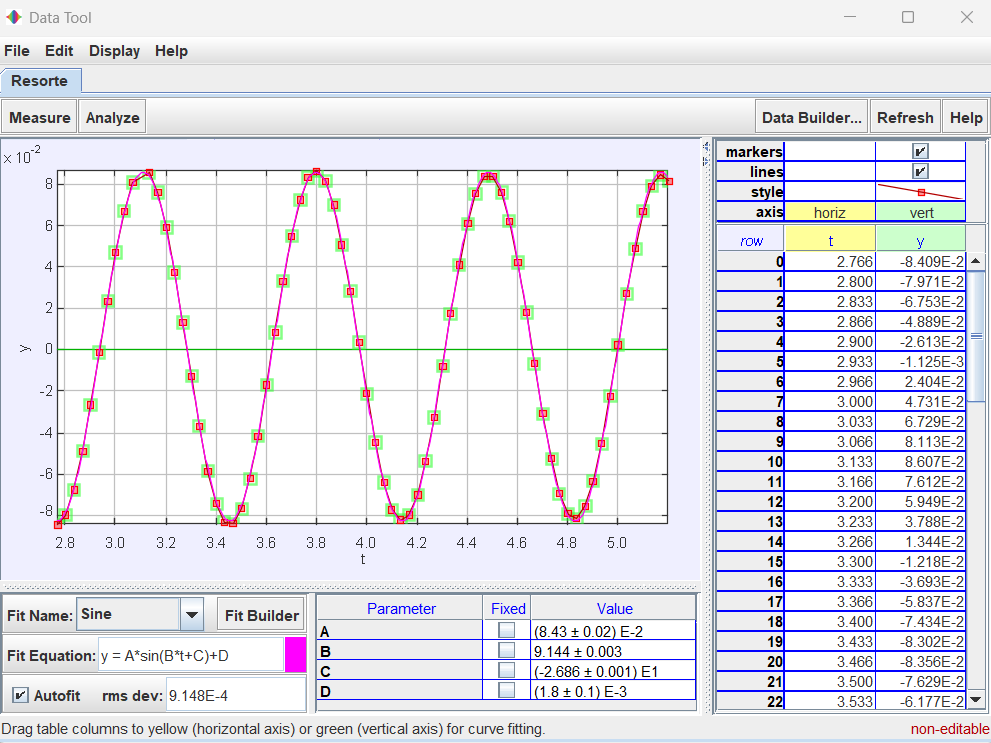
\includegraphics[scale=0.75]{Resorte.png}
    \caption{Gráfica de resorte}
    \label{Resorte}
\end{figure}
Usando (1) sacamos el promedio del período y de la Amplitud y obtenemos:
\begin{table}[H]
    \centering
    \begin{tabular}{|c|c|}
    \hline
        Periodo  & $0.687 \pm 0.001 s$ \\ \hline
        Amplitud & $8.43 \pm 1 cm $ \\ \hline        
    \end{tabular}
    \caption{Promedio}
    \label{Promedio}
\end{table}

Usando estos datos, (3) y sus derivaciones obtenemos:
(Usamos x en cm, y los ángulos en radianes)
\[x(t)=8.43sin(\frac{2\pi}{0.687} t -0.46879544)\]
\[v(t)=8.43\frac{2\pi}{0.687}cos(\frac{2\pi}{0.687} t -0.46879544)\]
\[a(t)=-8.43{(\frac{2\pi}{0.687})}^2sen(\frac{2\pi}{0.687} t -0.46879544)\]

Ahora, usando (7), obtenemos la constante del resorte calculada con la información obtenida del Tracker. Así calculamos: k=0.41823.

Usando (2) obtenemos un error porcentual de: e=15.423\%.

Para los otros movimientos, usando el mismo procedimiento de análisis con el Tracker y tenemos: para el péndulo físico:

\begin{figure} [H] 
    \centering
    \includegraphics[scale=0.5]{Péndulo.png}
    \caption{Gráfica de péndulo}
    \label{Péndulo}
\end{figure}

Y obtenemos una ecuación del movimiento (cm y rad):

\[x(t)=39.95sin(\frac{2\pi}{1.2371} t -0.181166)\]
\[v(t)=39.95\frac{2\pi}{1.2371}cos(\frac{2\pi}{1.2371} t -0.181166)\]
\[a(t)=-39.95(\frac{2\pi}{1.2371})^2sen(\frac{2\pi}{1.2371} t -0.181166))\]

Y por último, para el movimiento de la oscilación de la regla:

\begin{figure} [H] 
    \centering
    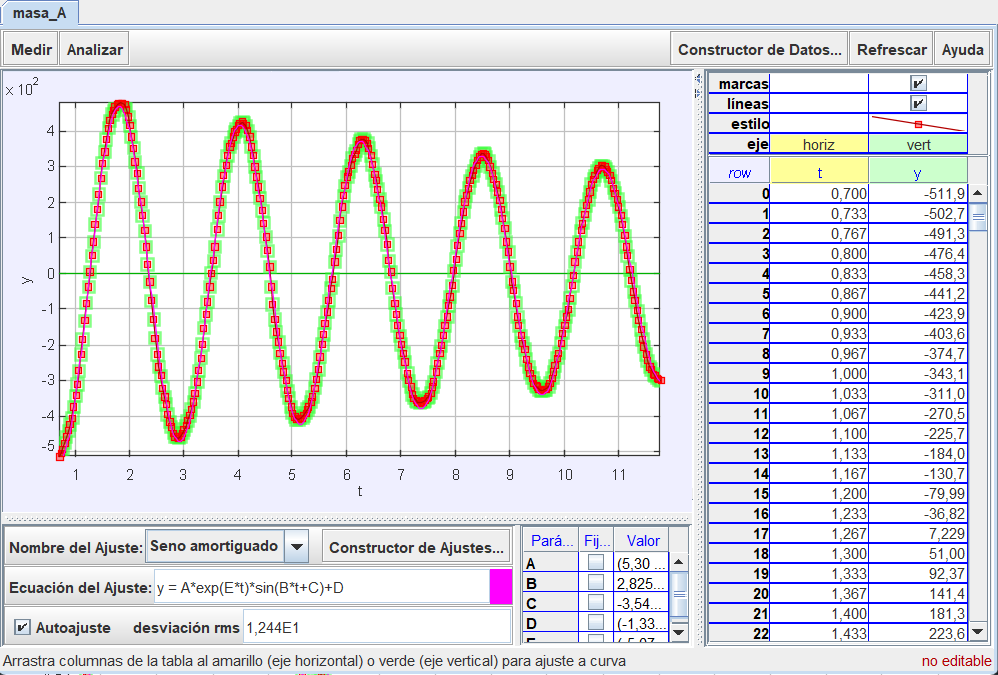
\includegraphics[scale=0.5]{Regla.png}
    \caption{Gráfica de la regla}
    \label{Regla}
\end{figure}

\section{Conclusiones}
Como se pudo observar en la práctica, el movimiento armónico aparece en muchos fenómenos físicos importantes, este tipo de movimiento se espera encontrar de una u otra manera en cualquier sistema porque es un movimiento relativamente sencillo de modelizar. El objetivo de esta práctica fue cumplido con éxito y se pudo modelizar con ayuda del Tracker los diferentes movimientos y calcular el error de la constante de elasticidad entre dos métodos experimentales distintos.

\section{Referencias}

\begin{enumerate}
    \item Herrera, N., Procel, L. (2018). \textit{Movimiento armónico simple}.
\end{enumerate}

\section{Anexos}

\begin{table}[H]
    \centering
    \begin{tabular}{|l|l|l|l|l|l|l|l|l|l|l|l|}
    \hline
        masa (gramos) & 0 & 150 & 200 & 250 & 300 & 350 & 400 & 450 & 500 & 520 & 540  \\ \hline
        elongacion (mm) & 58 & 84 & 109 & 134 & 157 & 179 & 209 & 235 & 258 & 264 & 277  \\ \hline
    \end{tabular}
    \caption{Datos para encontrar la constante elástica}
\end{table}

Evidencias de los videos:

\begin{figure} [H] 
    \centering
    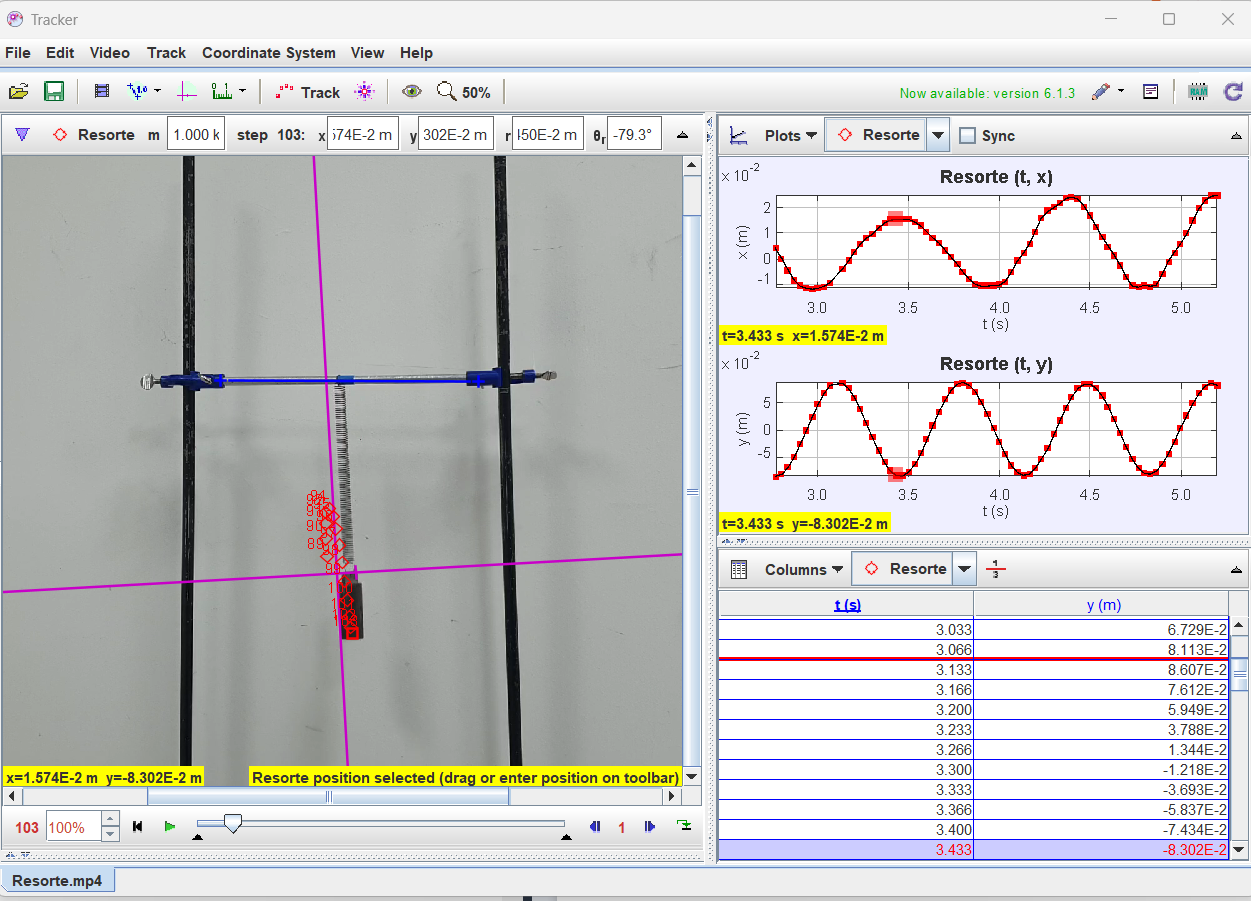
\includegraphics[scale=0.5]{Resorte 2.png}
    \caption{Gráfica de resorte evidencia}
    \label{Resorte 2}
\end{figure}

\begin{figure} [H] 
    \centering
    \includegraphics[scale=0.25]{Péndulo 2.png}
    \caption{Gráfica de péndulo evidencia}
    \label{Péndulo 2}
\end{figure}

\begin{figure} [H] 
    \centering
    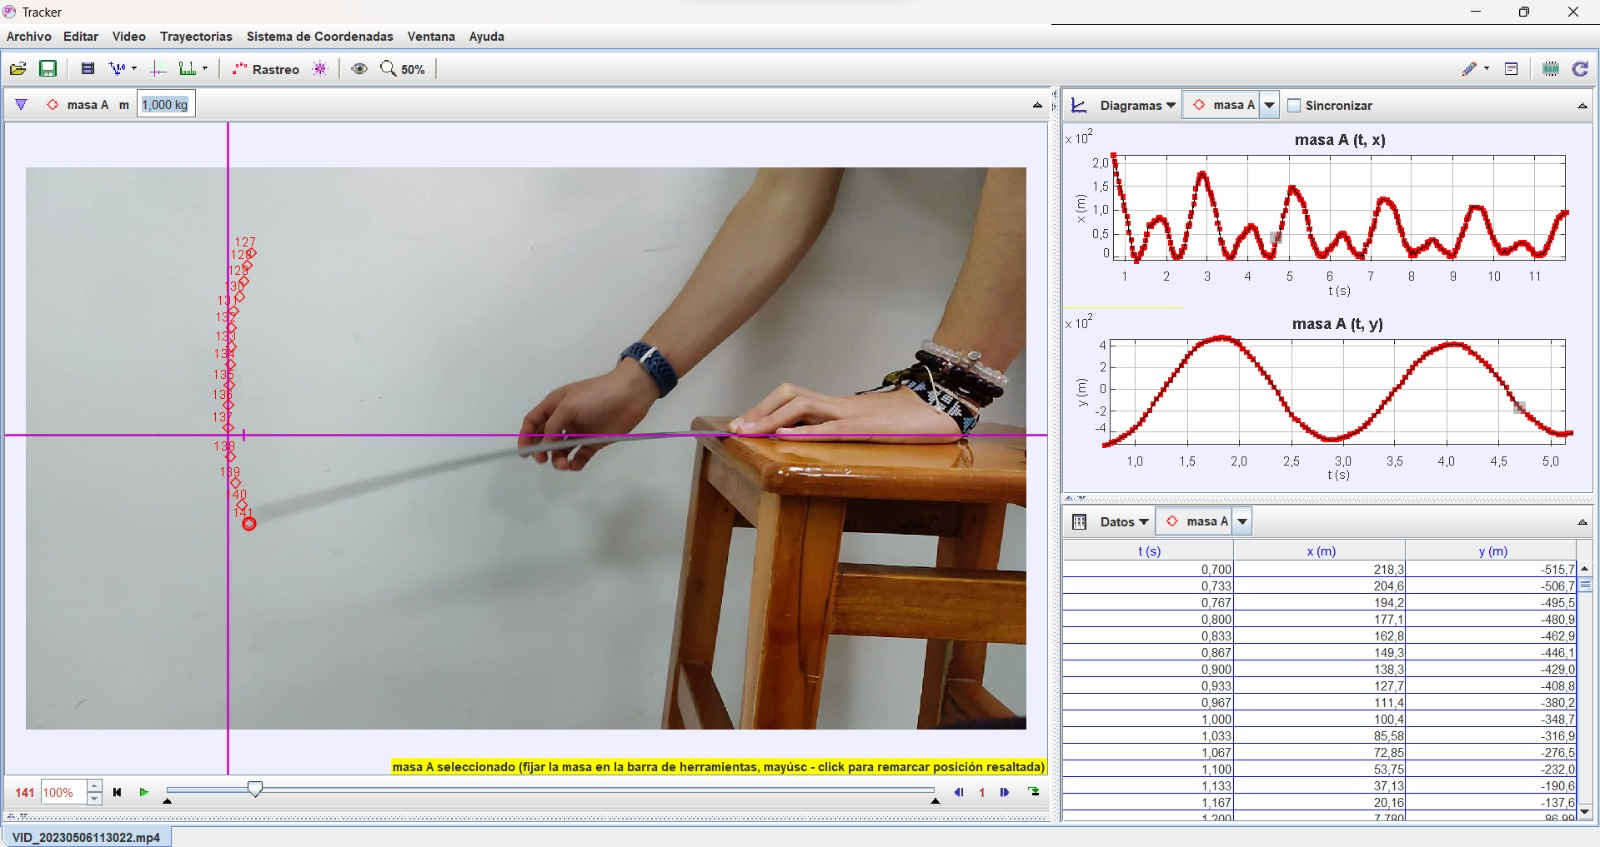
\includegraphics[scale=0.25]{Regla 2.png}
    \caption{Gráfica de regla evidencia}
    \label{Regla 2}
\end{figure}



\end{document}